\chapter{Introduction}

\section{Background on Solid-State Batteries}
The unprecedented demand for high-energy, safe, and long-lasting energy storage devices, driven by the proliferation of portable electronics and electric vehicles, has established lithium-ion batteries (LIBs) as the dominant technology. Conventional LIBs, however, rely on organic liquid electrolytes, which pose significant safety risks due to their inherent flammability and volatility. Furthermore, the use of liquid electrolytes can lead to the formation of lithium dendrites during fast charging or at low temperatures, creating pathways for internal short circuits that can result in thermal runaway \cite{Manthiram2017}. These safety concerns, coupled with the limited electrochemical window of liquid electrolytes, constrain the achievable energy density and operational lifespan of current battery systems.

To overcome these fundamental limitations, solid-state batteries (SSBs) have emerged as a transformative next-generation technology \cite{Janek2016}. SSBs replace the flammable liquid electrolyte with a solid-state electrolyte (SE), a move that promises to significantly enhance battery safety. The non-flammable nature of inorganic SEs intrinsically mitigates the risk of fire and explosion. Moreover, a mechanically robust SE can act as a physical barrier to suppress the growth of lithium dendrites, thereby enabling the use of a high-capacity lithium metal anode. This substitution is critical for pushing the energy density of batteries beyond the theoretical limits of conventional graphite anodes \cite{Famprikis2019}. The development of a suitable SE with high ionic conductivity, however, remains the central challenge hindering the widespread commercialization of SSBs, a problem that this thesis aims to address through computational methods.

\section{Working Principle and Advantages over Organic Electrolytes}

A solid-state battery operates on the same fundamental electrochemical principles as a conventional lithium-ion battery. It consists of an anode (the negative electrode), a cathode (the positive electrode), and an electrolyte that separates them. During discharge, lithium ions migrate from the anode, through the solid electrolyte, to the cathode, while electrons travel through the external circuit to generate an electric current. The process is reversed during charging. The critical distinction lies in the nature of the electrolyte; instead of a liquid organic solvent with dissolved lithium salts, an SSB utilizes a solid, ion-conducting material \cite{Bachman2016}. The efficiency of this process hinges on the ability of the solid electrolyte to facilitate rapid ion transport while blocking the passage of electrons, a property known as high ionic conductivity.

The replacement of the liquid component with a solid one offers several transformative advantages, as illustrated in Figure \ref{fig:ssb_vs_lib}.

\begin{itemize}
    \item \textbf{Enhanced Safety:} The primary advantage is the significant improvement in safety. Inorganic solid electrolytes are non-flammable and thermally stable, virtually eliminating the risk of fire or explosion associated with the volatile and flammable organic solvents used in traditional LIBs \cite{Manthiram2017}. This inherent safety profile is a crucial driver for their adoption in applications like electric vehicles and large-scale grid storage.

    \item \textbf{Higher Energy Density:} SSBs have the potential to deliver a step-change in energy density. The high mechanical strength of certain solid electrolytes can physically suppress the formation and growth of lithium dendrites. This enables the use of a high-capacity lithium metal anode, which has been termed the "holy grail" of battery research, in place of the lower-capacity graphite anodes used today. Furthermore, the wide electrochemical stability window of many solid electrolytes allows for their pairing with high-voltage cathode materials, further boosting the overall cell energy density \cite{Kato2016}.

    \item \textbf{Longer Cycle Life and Durability:} By eliminating the liquid electrolyte, SSBs can avoid many of the degradation mechanisms that plague conventional LIBs, such as the continuous formation of an unstable solid-electrolyte interphase (SEI) layer and side reactions between the electrolyte and the electrodes. This leads to a more stable system with the potential for a longer cycle life and improved calendar aging characteristics over a wider operational temperature range \cite{Famprikis2019}.

    \item \textbf{Design and Packaging Flexibility:} The all-solid-state construction removes the need for bulky containment and cooling systems associated with liquid electrolytes. This allows for more simplified and compact battery pack designs. It also enables novel cell architectures, such as bipolar stacking, where cells are stacked directly on top of each other without individual packaging, leading to higher volumetric energy density at the pack level.
\end{itemize}

The realization of these advantages is fundamentally dependent on discovering a solid electrolyte material that possesses a combination of high ionic conductivity, good chemical and electrochemical stability, and manufacturability.

% --- Suggested Image ---
\begin{figure}[h!]
    \centering
    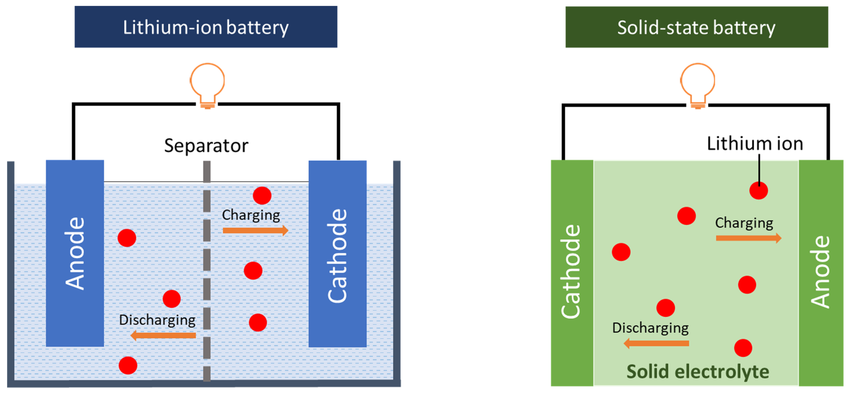
\includegraphics[width=0.8\textwidth]{Images/SSB-vs-LIB-structural-comparison.png}
    \caption{Comparison of a conventional lithium-ion battery (LIB) with a solid-state battery (SSB). The LIB (left) uses a liquid electrolyte and separator, which is susceptible to dendrite formation. The SSB (right) uses a dense solid electrolyte that blocks dendrites, enabling the use of a lithium metal anode.}
    \label{fig:ssb_vs_lib}
\end{figure}

\subsection{Motivation for Current Research}

Despite the immense promise of solid-state batteries, their widespread adoption is fundamentally gated by the discovery of a solid electrolyte material that satisfies a stringent set of requirements. Chief among these is achieving high ionic conductivity at room temperature, ideally on par with or exceeding that of conventional liquid electrolytes (i.e., > 1 mS/cm) \cite{Famprikis2019}. The search for such materials, however, represents a formidable challenge in materials science. The chemical space of potential inorganic solids is practically infinite, and exploring it through traditional methods is a slow and arduous process.

Experimental synthesis and characterization of novel materials is a resource-intensive endeavor, often described as a "trial-and-error" process that can take months or even years to yield a single promising candidate. On the computational front, first-principles methods like Density Functional Theory (DFT) can provide accurate predictions of ionic conductivity, but these calculations are computationally expensive and typically limited to a few hundred atoms, making them unsuitable for large-scale screening of thousands of potential candidates \cite{Zhu2015}. This "discovery bottleneck" significantly impedes the pace of innovation in solid-state electrolytes.

In recent years, data-driven approaches, specifically machine learning (ML), have emerged as a powerful new paradigm for accelerating materials discovery \cite{Butler2018}. By learning complex relationships from existing materials data, ML models can rapidly predict the properties of new, unseen materials at a fraction of the computational cost of first-principles methods. This high-throughput screening capability allows researchers to navigate the vast chemical space efficiently, identifying and prioritizing the most promising candidates for further investigation. The motivation for this thesis is therefore to leverage machine learning to bypass the traditional discovery bottleneck. Specifically, this work focuses on developing a predictive model for ionic conductivity that relies solely on readily available elemental properties, avoiding the need for computationally expensive structural information. Such a model provides an ultra-fast, structure-agnostic screening tool, enabling the rapid identification of novel solid electrolyte compositions worthy of more detailed experimental and computational study.

\subsection{Thesis Objectives and Outline}

The primary goal of this thesis is to develop and validate a machine learning framework for the rapid and accurate prediction of ionic conductivity in crystalline solid electrolytes. This work aims to establish a computationally inexpensive screening tool that can guide and accelerate the discovery of novel materials for solid-state battery applications. The specific objectives are as follows:

\begin{enumerate}
    \item To compile and process a comprehensive dataset of known solid electrolytes from the Database of Doped Solid Electrolytes (DDSE) \cite{DDSE2021} to serve as the foundation for model training and validation.
    \item To engineer a set of descriptive features based solely on the fundamental properties of the constituent elements of the materials, thereby creating a structure-agnostic predictive model.
    \item To train, optimize, and evaluate several machine learning regression models to identify the most effective algorithm for predicting ionic conductivity based on the engineered features.
    \item To analyze the performance of the best-performing model and interpret its predictions, validating the efficacy of the elemental-property-based approach for high-throughput screening of solid electrolytes.
\end{enumerate}

This thesis is structured as follows. Chapter 2 provides a comprehensive literature review on the state-of-the-art in solid electrolyte research, covering experimental techniques, first-principles calculations, and the growing application of machine learning in materials science. Chapter 3 details the methodology of this study, including the data collection process, the feature engineering strategy, and the implementation of the machine learning models. Chapter 4 presents and discusses the results of the predictive modeling, including model performance metrics and an analysis of feature importance. Finally, Chapter 5 concludes the thesis by summarizing the key findings, acknowledging the limitations of the current work, and outlining promising directions for future research.
